\section{Secțiune}

\begin{frame}{Secțiune: Componente Disponibile} \pause
	\begin{itemize}
		\item Repetarea în acest proiect a majorității componentelor definite în proiectul lucrării scrise \pause
		\item În continuare, numai exemple succinte de utilizare
	\end{itemize}
\end{frame}

\begin{frame}{Secțiune: Exemple de Componente I} \pause
	\begin{itemize}
		\item Un item \pause
		    \begin{itemize}
		        \item Un item imbricat \pause
		        \item Unul dintre itemii imbricați \pause
	        \end{itemize}
		\item Un alt item
	\end{itemize}
\end{frame}

\begin{frame}{Secțiune: Exemple de Componente II}
	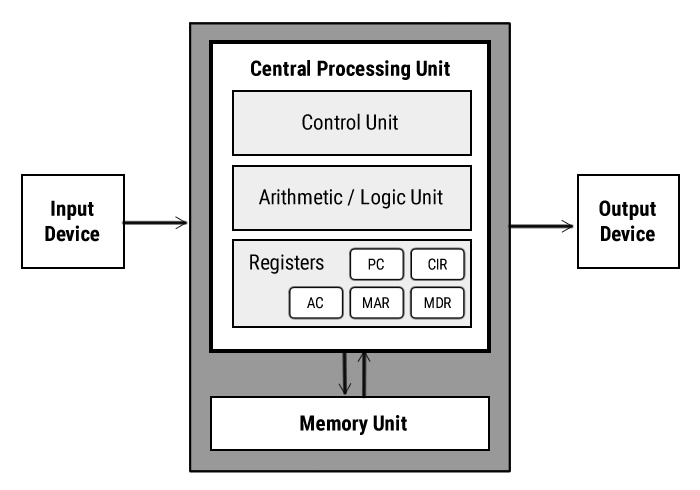
\includegraphics[width=0.8\textwidth, center]{components/images/architecture.jpg}
    \captionsetup{justification=centering,margin=1cm}
    \captionof{figure}{Arhitectura unui calculator}
\end{frame}

\begin{frame}{Secțiune: Exemple de Componente III}
	\begin{table}[h]
    \begin{tabular}{ | p{0.5\linewidth} | p{0.5\linewidth} | }
        \hline
        Nume Complet & Funcție Ocupată \\
        \hline
        Joshua Roob & Manager de Proiect \\
        Asa Hauck & Artist Grafic \\
        Harley Hagenes & Programator \\
        \hline
    \end{tabular}
    \caption{Colaboratori la Realizarea Studiului}
    \label{tab:small_table}
\end{table}
\end{frame}